\documentclass{beamer}
\usetheme{metropolis}
\usepackage{graphicx}
\usepackage{subfig}
\title{Safe Return Doubtful: History and Current Status of Modern Science in Antarctica}
\date{\today}
\author{Jordan Hanson}
\institute{Whittier College Department of Physics and Astronomy}

\begin{document}
\maketitle

\section{Opening Remarks - Exploration}

\begin{frame}{Opening Remarks - Exploration}
\textit{``We shall not cease from exploration \\
And the end of all our exploring \\
Will be to arrive where we started \\
And know the place for the first time.''} \\  \vspace{1cm} \textbf{T.S. Eliot, \textit{Little Gidding}, from  \textit{Four Quartets}, 1936-42.}
\end{frame}

\section{Summary}

\begin{frame}{Unit 0 Summary}
\begin{enumerate}
\item Why explore?
\begin{itemize}
\item \textit{Little Gidding}, secs. IV and V
\item You \textit{can} explore, but why?
\item The other part...
\end{itemize}
\item Course syllabus
\item The books and journal
\item Warm up exercises: mileage
\item Force, energy, work, and friction
\item Unit conversions
\begin{itemize}
\item Currency
\item Energy
\end{itemize}
\item \textbf{The extent of the Solar System, part I}
\end{enumerate}
\end{frame}

\section{Why Explore?}

\begin{frame}{Why Explore?}
\textbf{Why explore?}
\begin{enumerate}
\item The world is a beautiful place
\item To learn things you do not know that you do not know
\item To learn about about yourself
\end{enumerate}
\end{frame}

\begin{frame}{Why Explore?}
\textbf{That other part...}
\begin{enumerate}
\item How to handle yourself in strange situations
\item How to use your brain to survive
\item \textit{What really matters}
\end{enumerate}
\end{frame}

\section{Warm-up exercises}

\begin{frame}{Warm-ups}
\begin{enumerate}
\item How many gallons of gasoline will your vehicle hold?  (Or that of your family, friends).
\item What is the gas mileage on the highway?
\item How far can you go?
\end{enumerate}
\end{frame}

\section{Unit Conversions}

\begin{frame}{Unit Conversions}
We must learn how to deal with \textit{units.}
\begin{enumerate}
\item In 1900-1915, 1.0 USD equals 3.8 krone.
\item One Calorie, which equals 1 kilocalorie, is 4184 \textit{Joules}.
\end{enumerate}
\end{frame}

\begin{frame}{Unit Conversions}
\small
We must learn how to deal with \textit{units.}
\begin{enumerate}
\item \textbf{In 1900-1915, 1.0 USD equals 3.8 krone.}
\item One Calorie, which equals 1 kilocalorie, is 4184 \textit{Joules}.
\end{enumerate}
Question - The \textit{Primus stove} was invented in 1892 by Franz Wilhelm Lindqvist, from Sweden.  Suppose it cost 12.00 krone.  What did it cost in USD? \\ \vspace{0.5cm}
Question - A northern sled dog was required for sledging in the early 1900s.  Suppose one could be purchased for 50.00 USD.  What is that cost in krone? \\
\end{frame}

\begin{frame}{Unit Conversions}
\small
We must learn how to deal with \textit{units.}
\begin{enumerate}
\item In 1900-1915, 1.0 USD equals 3.8 krone.
\item \textbf{One Calorie, which equals 1 kilocalorie, is 4184 \textit{Joules}.}
\end{enumerate}
Question - An inactive person requires about 2000 Calories per day.  How many Joules does she require per day?  \\ \vspace{0.5cm}
Question - A typical source of protein contains 4.0 Calories per gram.  How many Joules are in 200 grams of protein? \\
\end{frame}

\section{Force, Work, and Energy}

\begin{frame}{Force, Work, and Energy}
\textbf{Force:} 
\begin{equation}
F = m a
\end{equation}
\begin{itemize}
\item F: Force, in Newtons (British unit: pounds or lbs.)
\item m: mass, in kilograms (British unit: stone)
\item a: acceleration, in meters per second squared (British unit: feet per second squared)
\end{itemize}
\textbf{Professor: work several examples.}
\end{frame}

\begin{frame}{Force, Work, and Energy}
\textbf{Work, or energy:} 
\begin{equation}
W = F d
\end{equation}
\begin{itemize}
\item F: Force, in Newtons (British unit: pounds or lbs.)
\item d: Distance, in meters (British unit: feet)
\end{itemize}
\textbf{Professor: work several examples.}
\end{frame}

\begin{frame}{Force, Work, and Energy}
\textbf{Force of friction:} 
\begin{equation}
f = \mu m g
\end{equation}
\begin{itemize}
\item f: Force of friction, in Newtons (British unit: pounds or lbs.)
\item $\mu$: Greek letter mu, unit-less constant ($\approx 0.01 - 0.1$)
\item g: acceleration downward due to gravity, or 9.81 meters per second squared.
\end{itemize}
\textbf{Professor: work several examples.}
\end{frame}

\section{Warm-up exercises}

\begin{frame}{Warm-ups}
\begin{enumerate}
\item How many kcal do you eat per day? (Pick a number between 2000 and 4000).
\item How much energy is this in Joules?
\item A unit of \textit{power} is a Joule per second (J/s), also known as a Watt:
\begin{equation}
Power = \frac{Energy}{time}
\end{equation}
\item Suppose running at 4 m/s requires 1000 Watts.  For how long can you run with the amount of energy you picked in step 1?
\end{enumerate}
\end{frame}

\begin{frame}{Warm-ups}
\begin{enumerate}
\item Recall that 
\begin{equation}
velocity = \frac{distance}{time}
\end{equation}
Taking your answer from the previous question for the time you can run at 4 m/s on the energy you consume, predict how \textit{far} you can run at 4 m/s before running out of energy.
\item What if at this distance there was a \textit{depot} of food, containing an additional 2000 kcal of energy.  Suppose you consume it.  How much farther can you go?
\end{enumerate}
\end{frame}

\section{Astronomy and Early Antarctic Exploration}

\begin{frame}{Astronomy and Early Antarctic Exploration}
James Cook and Charles Green, 1769
\begin{enumerate}
\item Kepler's Laws: $T^2 \propto r^3$
\item Kepler: Preduicted when Venus would \textit{transit} the Sun, from our perspective
\item What is an AU?
\item Sir Edmond Halley (1656 - 1742).  Halley's comet passed by in 1758 (16 years after he died).
\begin{itemize}
\item Devised a method for determining distance to the Sun.
\item Astronomers sent out all over the world (Baja California, Tahiti, etc.) to make the recordings.
\end{itemize}
\end{enumerate}
It is worth noting that an early Polynesian explorer is claimed by the Maori to have seen Antarctica first: \url{https://en.wikipedia.org/wiki/Ui-te-Rangiora}
\end{frame}

\begin{frame}{Astronomy and Early Antarctic Exploration}
What are Kepler's Laws?
\begin{enumerate}
\item \textbf{The Law of Orbits}: All planets move in elliptical orbits, with the sun at one focus.
\item \textbf{The Law of Areas}: A line that connects a planet to the sun sweeps out equal areas in equal times.
\item \textbf{The Law of Periods}: The square of the period of any planet is proportional to the cube of the semimajor axis of its orbit.
\end{enumerate}
\end{frame}

\begin{frame}{Astronomy and Early Antarctic Exploration}
\small
\textbf{The Law of Orbits}: All planets move in elliptical orbits, with the sun at one focus.
\begin{figure}
\centering
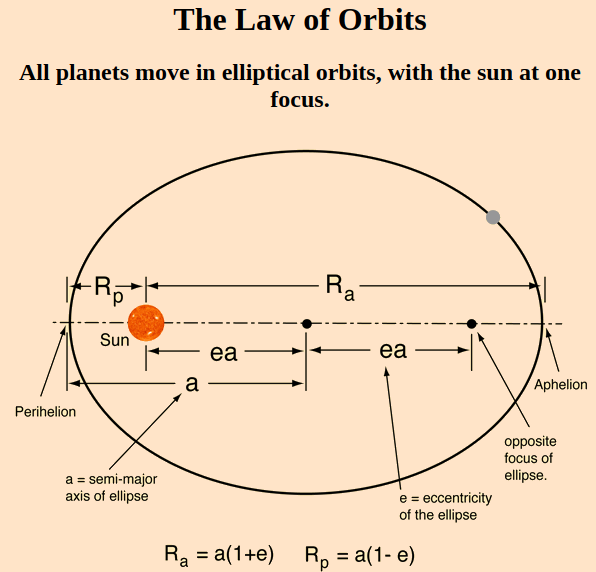
\includegraphics[width=0.5\textwidth]{figures/orbit1.png}
\caption{\label{fig:orbit1} A diagram describing Kepler's First Law.  A circle is a special case of an ellipse.}
\end{figure}
\end{frame}

\begin{frame}{Astronomy and Early Antarctic Exploration}
\small
\textbf{The Law of Areas}: A line that connects a planet to the sun sweeps out equal areas in equal times.
\begin{figure}
\centering
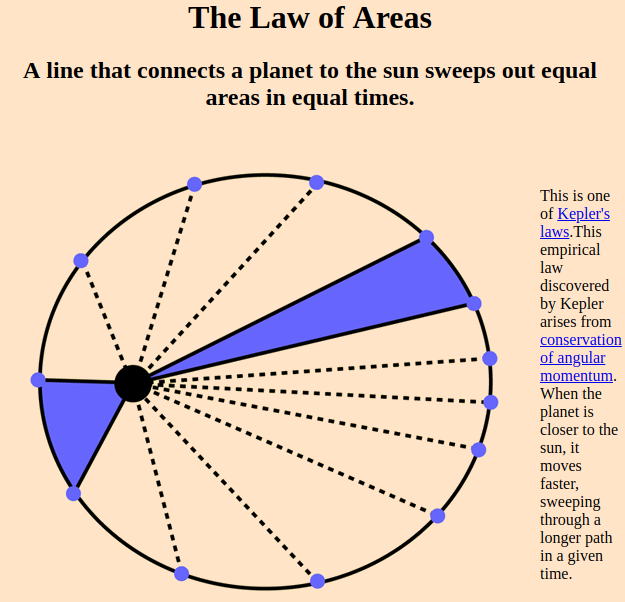
\includegraphics[width=0.5\textwidth]{figures/orbit2.png}
\caption{\label{fig:orbit2} A diagram describing Kepler's Second Law.  Areas are swept out in equal times.}
\end{figure}
\end{frame}

\begin{frame}{Astronomy and Early Antarctic Exploration}
\small
\textbf{The Law of Periods}: The square of the period of any planet is proportional to the cube of the semimajor axis of its orbit.
\begin{figure}
\centering
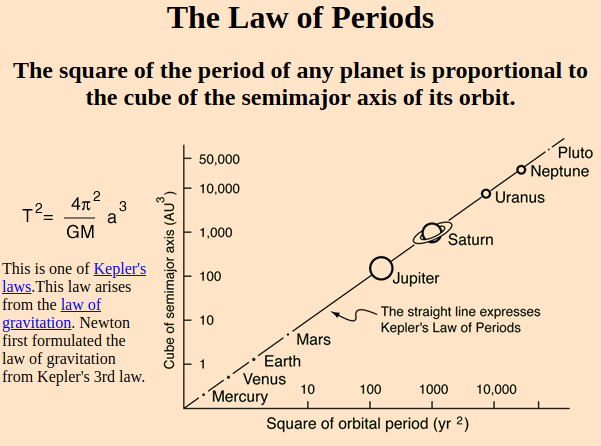
\includegraphics[width=0.5\textwidth]{figures/orbit3.png}
\caption{\label{fig:orbit3} A diagram describing Kepler's Third Law.  Period squared is proportional to radius cubed.}
\end{figure}
\end{frame}

\begin{frame}{Astronomy and Early Antarctic Exploration}
\small
How can we use Kepler's Third Law to understand the location of the planets with respect to the Sun?
\begin{equation}
T^2 \propto r^3
\end{equation}
Can we use geometry to determine $r$ for a planet independently?
\end{frame}

\begin{frame}{Astronomy and Early Antarctic Exploration}
\small
\begin{figure}
\centering
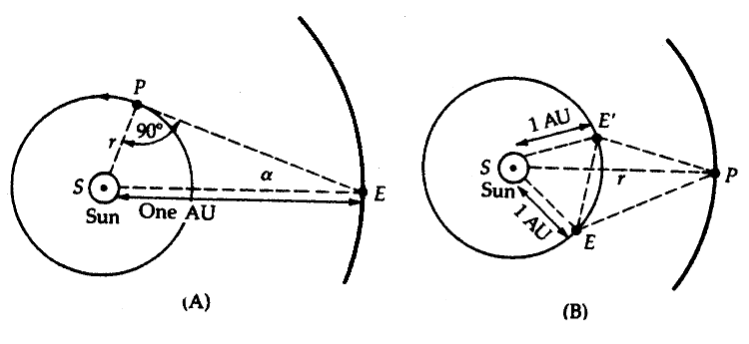
\includegraphics[width=0.9\textwidth]{figures/orbit4.png}
\caption{\label{fig:orbit4} A diagram describing how Kepler determined radii.  (Left) the method for a planet closer to the Sun that the Earth.  (Right) the method for a planet farther from the Sun than the Earth.}
\end{figure}
\textbf{Professor example: trigonometry for Venus.}
\end{frame}

\begin{frame}{Astronomy and Early Antarctic Exploration}
Result of measuring the elongation angle for Venus: 46 degrees. \\ \vspace{1cm}
Radius of Venus \textit{relative to that of the Earth:} 0.72 AU. \\ \vspace{1cm}
\textbf{What then is the period of Venus?} Use Kepler's Third Law, relative to Earth (observe on board).
\begin{equation}
\left(\frac{R_{E}}{R_{V}}\right)^2 = \left(\frac{T_{E}}{T_{V}}\right)^3
\end{equation}
$T_E$ is the quantity 1.0 year, and $R_E$ we do not know, but we simply call it 1 AU, or $R_{AU}$.
\end{frame}

\begin{frame}{Astronomy and Early Antarctic Exploration}
At your tables, fill in the following data using Kepler's Third Law:
\begin{table}
\centering
\begin{tabular}{| c | c | c |}
\hline \hline
Planet & Radius (AU) & Period \\
Mercury & 0.387 & -- \\ 
Venus & 0.723 & -- \\ 
Earth & 1.0 & 1.0 \\ 
Mars & 1.524 & -- \\ 
Jupiter & 5.203 & -- \\ 
Saturn & 9.537 & -- \\ 
Uranus & 19.191 & -- \\ 
Neptune & 30.069 & -- \\ 
\hline
\hline
\end{tabular}
\caption{\label{tab:kep} Table of orbits of the planets of our solar system.}
\end{table}
\end{frame}

\begin{frame}{Astronomy and Early Antarctic Exploration}
\small
In 1769, people did not know the amount of kilometers corresponding to 1 AU.  Sir Edmond Halley devised a method for determining the result, but it required transporting astronomers to opposite sides of the planet.  A short video describes the technique: \\ \vspace{0.5cm}
\url{https://youtu.be/GwP8wCzbFLc}
\begin{figure}
\centering
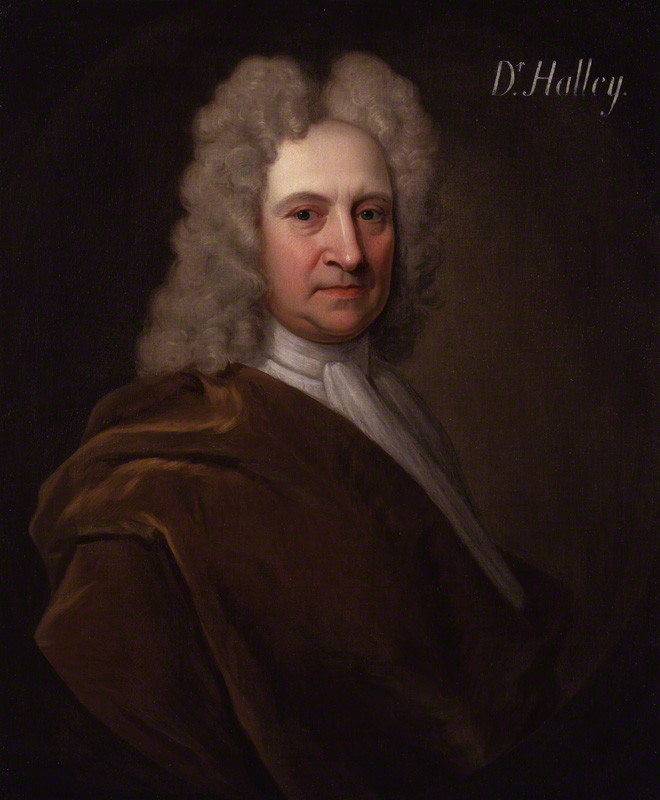
\includegraphics[width=0.25\textwidth]{figures/Edmond_Halley_072.jpg}
\caption{\label{fig:halley} Sir Edmond Halley (1656-1742) was the Royal Astronomer of Great Britain, and a colleague of Isaac Newton.}
\end{figure}
\end{frame}

\begin{frame}{Astronomy and Early Antarctic Exploration}
Definition of an angle \textit{in radians:}
\begin{equation}
s = r \theta
\end{equation}
Using this and other observations, we can show that
\begin{equation}
R_{AU} = \frac{D_E}{2\pi\Delta t \left( T_V^{-1} - T_E^{-1} \right)}
\end{equation}
\begin{itemize}
\item $D_E$ is Earth diameter 12,000 km
\item $\Delta t$ is about 12 minutes
\item $T$ values are orbital periods
\end{itemize}
\textbf{Let's try to derive the AU!}
\end{frame}

\section{Summary}

\begin{frame}{Unit 0 Summary}
\begin{enumerate}
\item Why explore?
\begin{itemize}
\item \textit{Little Gidding}, secs. IV and V
\item You \textit{can} explore, but why?
\item The other part...
\end{itemize}
\item Course syllabus
\item The books and journal
\item Warm up exercises: mileage
\item Force, energy, work, and friction
\item Unit conversions
\begin{itemize}
\item Currency
\item Energy
\end{itemize}
\item \textbf{The extent of the Solar System.}
\item Early Antarctic Exploration
\end{enumerate}
\end{frame}

\end{document}
